\documentclass[12pt,a4paper]{article}
\usepackage[utf8]{inputenc}
\usepackage[T1]{fontenc}
\usepackage[vietnamese]{babel}
\usepackage{geometry}
\geometry{
    a4paper,
    left=30mm,
    right=20mm,
    top=20mm,
    bottom=20mm
}
\usepackage{graphicx}
\usepackage{array}
\usepackage{amsmath}
\usepackage{booktabs}
\usepackage{color}
\usepackage[table,xcdraw]{xcolor}
\usepackage{caption}
\usepackage{enumitem}
\usepackage{indentfirst}
\usepackage{tabularx}
\usepackage{hyperref}

% Define colors matching the professional theme
\definecolor{navy}{HTML}{1B365D}
\definecolor{lightblue}{HTML}{336699}
\definecolor{tableheader}{HTML}{1B365D}
\definecolor{lightgray}{HTML}{F2F2F2}

\captionsetup{font=it, labelsep=colon}
\setlist[itemize]{noitemsep, topsep=3pt, parsep=3pt, partopsep=0pt}

\begin{document}

% --- Administrative Header ---
\begin{center}
    \textbf{\large CỘNG HÒA XÃ HỘI CHỦ NGHĨA VIỆT NAM}\\
    \textbf{\large Độc Lập - Tự Do - Hạnh Phúc}\\
    \small ---------------o0o---------------\\
    \vspace{2em}
    \textbf{\Large BẢN MÔ TẢ GIẢI PHÁP HỮU ÍCH}\\
    \vspace{1em}
    \textbf{\large Tên giải pháp: HỆ THỐNG DI ĐỘNG TƯƠNG TÁC THÔNG MINH GIÁM SÁT SỨC KHỎE GIẤC NGỦ VÀ TẦM SOÁT HỘI CHỨNG NGƯNG THỞ KHI NGỦ (SLEEPCARE)}
\end{center}

\vspace{1.5em}

\noindent Tên gọi sáng chế của phần mềm ứng dụng di động là \textbf{SleepCare (Hệ thống giám sát sức khỏe giấc ngủ và hỗ trợ tầm soát ngưng thở khi ngủ từ xa)}, là giải pháp phần mềm và kiến trúc tương tác do GS.TS.KH. Dương Quý Sỹ đề xuất bảo hộ quyền sở hữu trí tuệ, nhằm cung cấp giải pháp sàng lọc không xâm lấn dễ tiếp cận dưới sự hỗ trợ chuyên môn của Hội Y học Giấc ngủ Việt Nam.

% --- Section I ---
\section{\textcolor{navy}{I. THÔNG TIN CHUNG VÀ CỐ VẤN KHOA HỌC}}
\begin{itemize}
    \item \textbf{Cố vấn khoa học \& Chỉ đạo chuyên môn:} GS. TS. KH. Dương Quý Sỹ (\textit{Chủ tịch Hội Y học Giấc ngủ Việt Nam - VSSM}).
    \item \textbf{Đơn vị bảo trợ học thuật và đồng hành chuyên môn:} Hội Y học Giấc ngủ Việt Nam (VSSM).
    \item \textbf{Nhóm tác giả nghiên cứu chế tạo:} GS.TS.KH. Dương Quý Sỹ, ThS. Trần Hữu Nam, ThS. Nguyễn Tuấn Anh, ThS. Tăng Thị Thảo Trâm, CN. Trần Thị Cẩm Tú, DS. Nguyễn Trọng Bằng, ThS. Nguyễn Văn Tới, TS. Nguyễn Duy Thái, GS. Ramon Farré, GS.TS. Thomas Penzel, GS.TS. Francis Martin, GS. Đinh Xuân Anh Tuấn.
\end{itemize}

\begin{figure}[h!]
    \centering
    
\includegraphics[width=0.3\textwidth]{logo.png}
    \caption{Biểu tượng ứng dụng SleepCare được bảo trợ chuyên môn bởi Hội Y học Giấc ngủ Việt Nam.}
    \label{fig:logo}
\end{figure}

% --- Section II ---
\section{\textcolor{navy}{II. LĨNH VỰC KỸ THUẬT ĐƯỢC ĐỀ CẬP}}
Giải pháp hữu ích này đề cập đến lĩnh vực phần mềm y tế và thiết bị theo dõi sức khỏe cá nhân, cụ thể là hệ thống ứng dụng di động tương tác thông minh (SleepCare) tích hợp các thuật toán xử lý tín hiệu số thu được từ các cảm biến phần cứng có sẵn của điện thoại di động (microphone, cảm biến ánh sáng hoặc camera trước) nhằm giám sát chất lượng môi trường phòng ngủ, thu âm phân tích tiếng ngáy thời gian thực, thực hiện sàng lọc bệnh lý ngưng thở khi ngủ do tắc nghẽn (OSA) dựa trên các thang đo lâm sàng chuẩn hóa quốc tế và kết nối hệ thống y tế giấc ngủ.

% --- Section III ---
\section{\textcolor{navy}{III. TÌNH TRẠNG KỸ THUẬT CỦA GIẢI PHÁP HỮU ÍCH}}
Hội chứng ngưng thở khi ngủ do tắc nghẽn (OSA) là một bệnh lý hô hấp nguy hiểm liên quan mật thiết đến các nguy cơ tim mạch và đột quỵ. Tiêu chuẩn vàng để chẩn đoán OSA hiện nay là đo đa ký giấc ngủ (Polysomnography - PSG) tại các phòng thí nghiệm giấc ngủ chuyên dụng.

Tuy nhiên, việc triển khai chẩn đoán OSA gặp nhiều khó khăn do:
\begin{itemize}
    \item Chi phí thực hiện đo PSG tại phòng khám y tế lớn và đắt đỏ, đòi hỏi bệnh nhân phải ngủ lại qua đêm với nhiều dây cáp kết nối trên cơ thể gây khó chịu và thay đổi sinh lý giấc ngủ tự nhiên.
    \item Các ứng dụng di động theo dõi giấc ngủ thương mại hiện có chủ yếu dựa trên cảm biến gia tốc để ước lượng chu kỳ thức-ngủ chung chung, thiếu độ tin cậy y học và hoàn toàn không tích hợp các bộ câu hỏi lâm sàng chuẩn hóa.
    \item Thiếu các giải pháp sàng lọc không xâm lấn tại nhà có thể đo lường tiếng ngáy kết hợp với các thông số môi trường phòng ngủ (độ ồn, độ sáng) để đưa ra chỉ số cảnh báo rủi ro mang tính khoa học.
    \item Chưa có hệ thống kết nối trực tiếp giúp đồng bộ hóa dữ liệu sàng lọc ban đầu của bệnh nhân tại nhà với mạng lưới các chuyên gia và phòng khám giấc ngủ chuyên khoa của Hội Y học Giấc ngủ Việt Nam.
\end{itemize}

% --- Section IV ---
\section{\textcolor{navy}{IV. BẢN CHẤT KỸ THUẬT CỦA GIẢI PHÁP HỮU ÍCH}}
Để giải quyết các hạn chế trên, giải pháp hữu ích đề xuất hệ thống phần mềm di động SleepCare hoạt động trên các hệ điều hành iOS/Android với kiến trúc đa mô-đun tích hợp:

\begin{itemize}
    \item \textbf{Mô-đun bảng hỏi sàng lọc lâm sàng chuẩn hóa:} Số hóa bộ câu hỏi sàng lọc buồn ngủ ban ngày Epworth (ESS) và bộ câu hỏi đánh giá rủi ro ngưng thở khi ngủ STOP-BANG, kết hợp thông tin nhân trắc học (BMI) để tự động tính điểm rủi ro.
    \item \textbf{Mô-đun phân tích tiếng ngáy thời gian thực dựa trên AI:} Sử dụng mic của điện thoại thu âm luồng âm thanh PCM 16kHz, chạy mô hình phát hiện tiếng ngáy cục bộ (sử dụng thư viện \texttt{snore\_detection}) để đếm số cơn ngáy, thời lượng ngáy và phát hiện ngáy bệnh lý dựa trên cường độ âm thanh (>56 dB) kéo dài.
    \item \textbf{Mô-đun đánh giá chất lượng môi trường phòng ngủ (Room Quality):} Đo cường độ tiếng ồn phòng ngủ (dB) kết hợp cảm biến ánh sáng xung quanh (hoặc phân tích luồng ảnh camera trước làm phương án dự phòng) để tính toán độ sáng tối ưu cho giấc ngủ (Lux/Kelvin).
    \item \textbf{Mô-đun kết nối y khoa từ xa:} Đồng bộ hóa dữ liệu đo đa ký giấc ngủ tại nhà (Home PSG) và đăng ký lịch khám tại các phòng khám đạt tiêu chuẩn quốc gia của VSSM thông qua giao tiếp mạng thời gian thực.
\end{itemize}

\begin{figure}[h!]
    \centering
    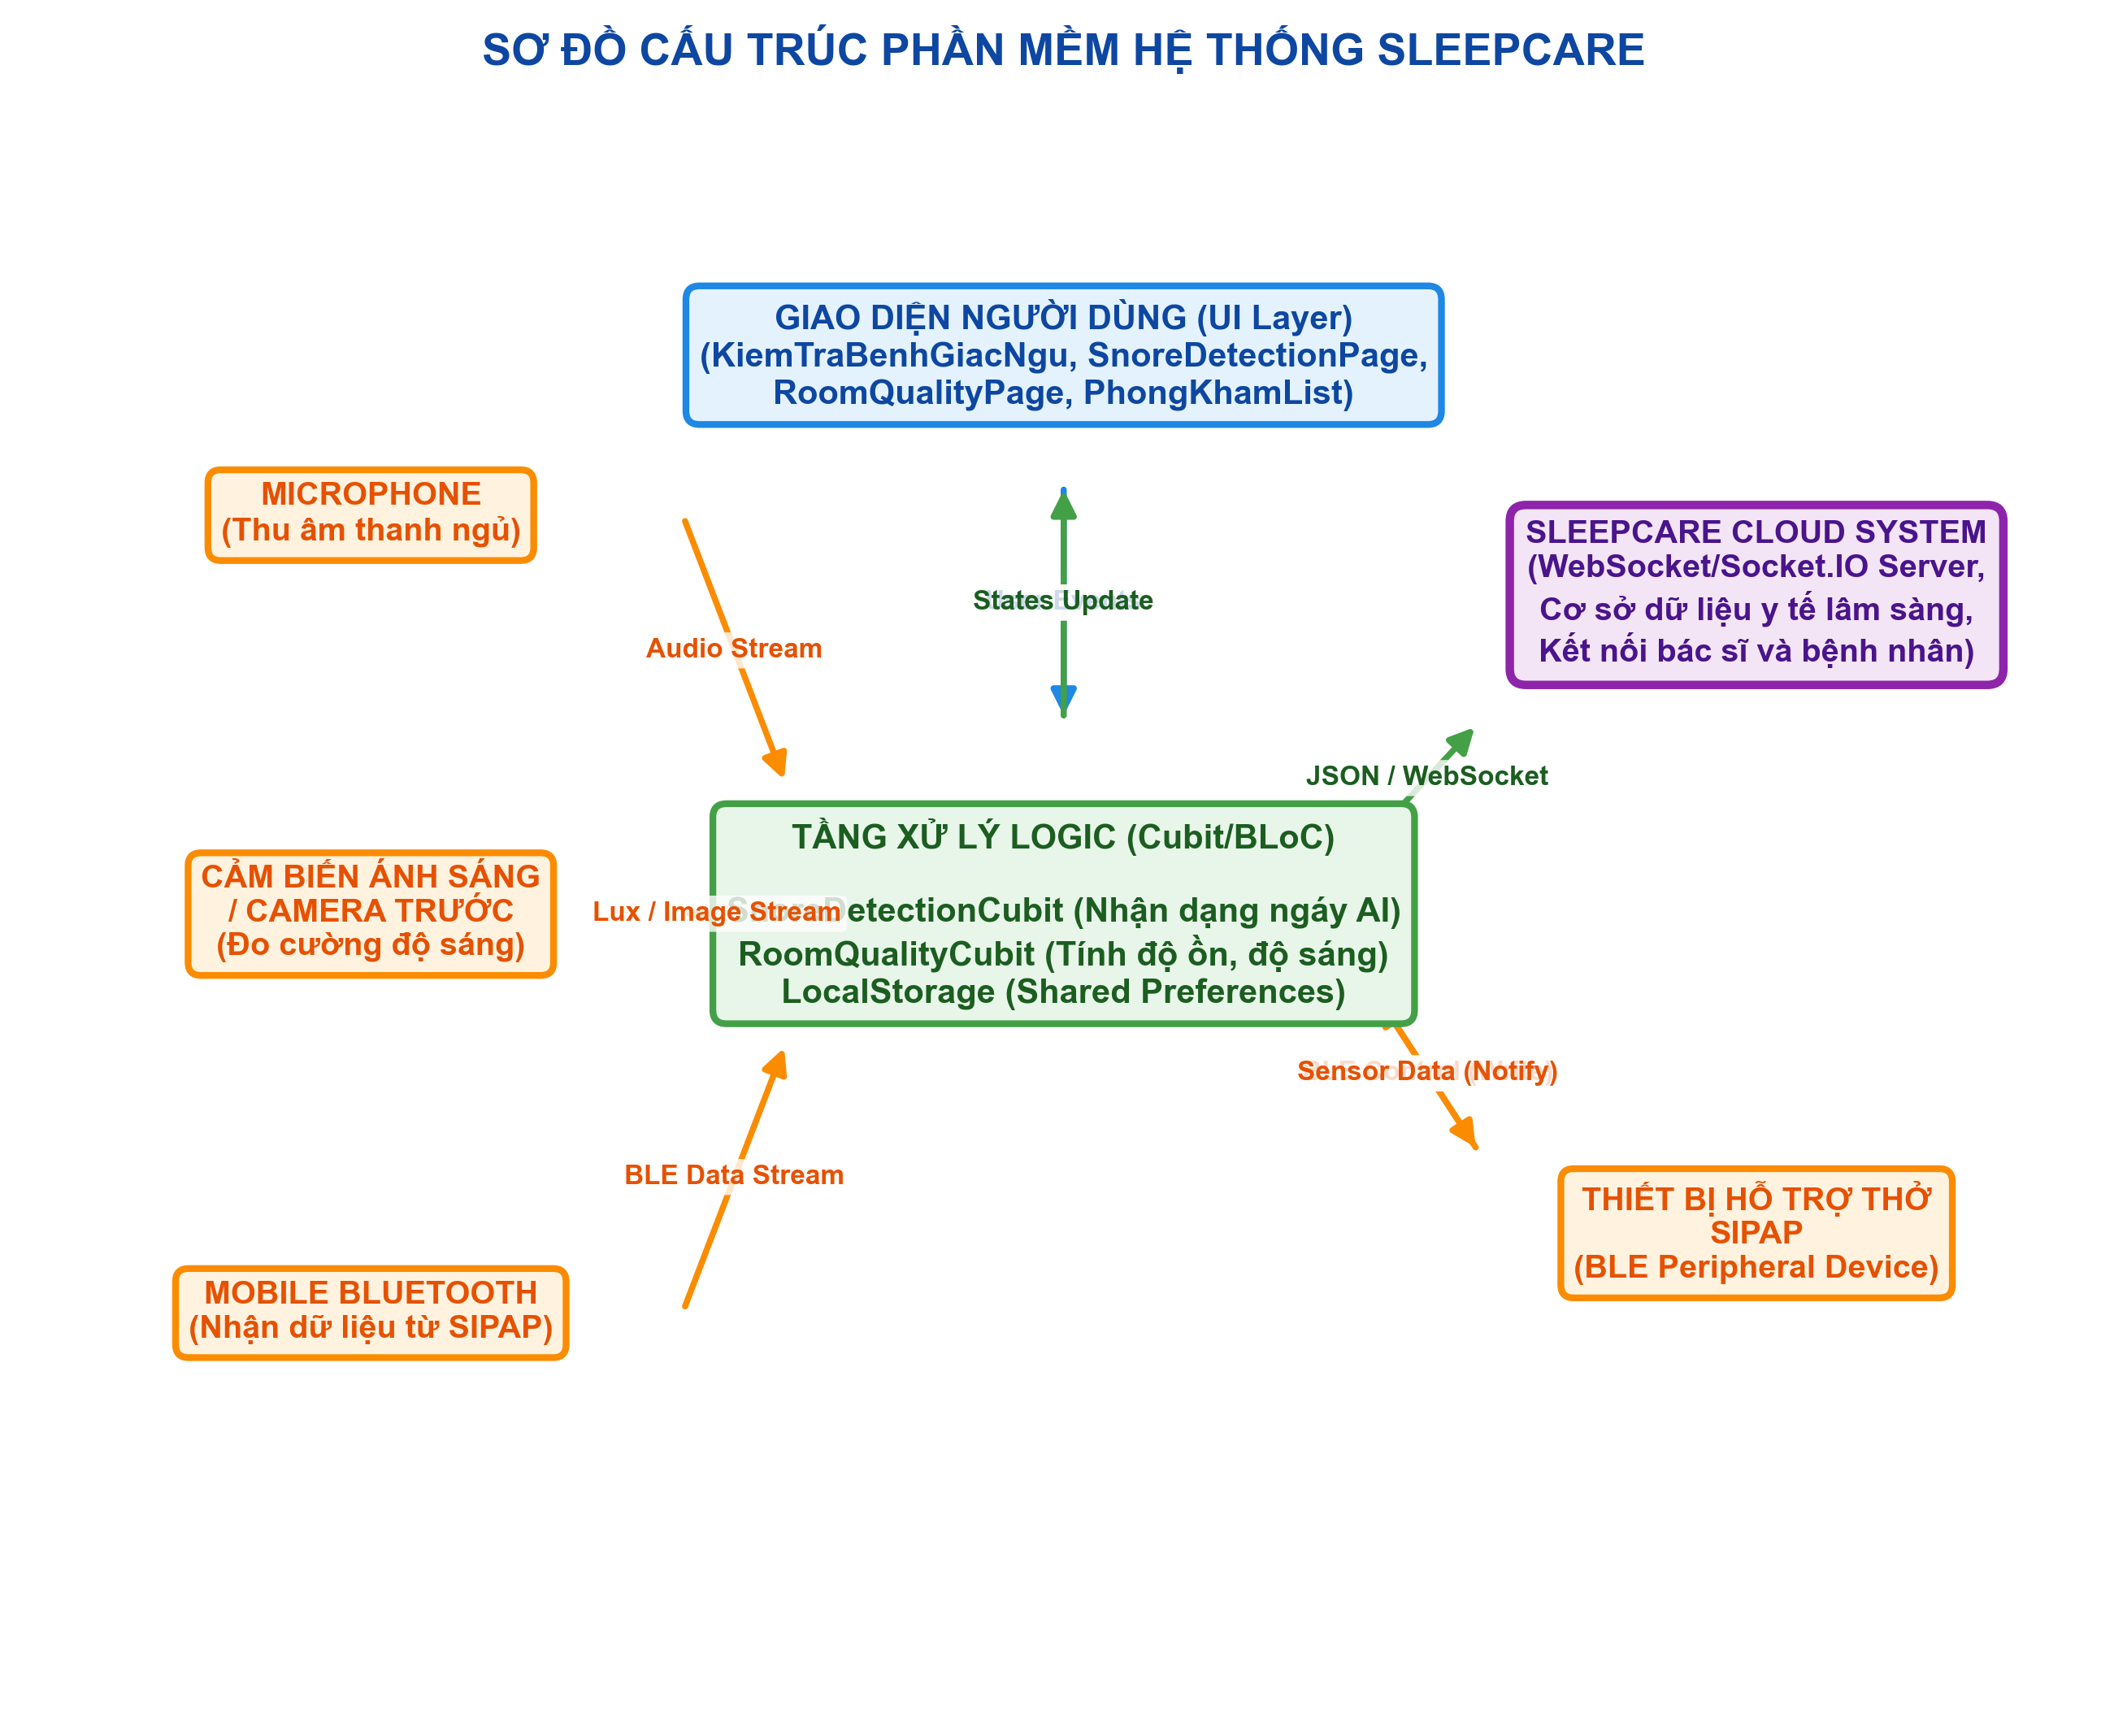
\includegraphics[width=0.8\textwidth]{sleepcare_architecture.png}
    \caption{Sơ đồ cấu trúc phần mềm và các khối kết nối tương tác của hệ thống SleepCare.}
    \label{fig:arch}
\end{figure}

% --- Section V ---
\section{\textcolor{navy}{V. MÔ TẢ CHI TIẾT PHƯƠNG ÁN THỰC HIỆN}}

\subsection{Sơ đồ cấu trúc phần mềm hệ thống}
Hệ thống được lập trình bằng ngôn ngữ Dart trên nền tảng Flutter, sử dụng kiến trúc quản lý trạng thái BLoC/Cubit để đảm bảo độ mượt mà và xử lý bất đồng bộ dữ liệu cảm biến:
\begin{itemize}
    \item \textbf{Tầng giao diện (UI Layer):} Cung cấp các trang màn hình: Sàng lọc rủi ro giấc ngủ (KiemTraBenhGiacNgu), Kiểm tra chất lượng phòng (RoomQualityPage), Đo tiếng ngáy (SnoreDetectionPage), Danh sách phòng khám chuyên khoa (PhongKhamList), và Giáo dục y khoa (ResourcesPage).
    \item \textbf{Tầng quản lý trạng thái (State Management):} Sử dụng \texttt{SnoreDetectionCubit} để điều phối thu âm stream và chạy mô hình AI; sử dụng \texttt{RoomQualityCubit} để đọc cảm biến ánh sáng và tính toán tiếng ồn môi trường.
    \item \textbf{Tầng dịch vụ (Service Layer):} Gồm kết nối WebSocket qua Socket.IO tới máy chủ trung tâm để truyền nhận dữ liệu lâm sàng thời gian thực, lưu trữ cục bộ qua Shared Preferences và đọc cấu hình động qua Firebase Remote Config.
\end{itemize}

\subsection{Chi tiết các thuật toán xử lý dữ liệu cảm biến}

\subsubsection*{a) Thuật toán phát hiện tiếng ngáy và tiếng ngáy bệnh lý}
Quá trình ghi âm và phát hiện tiếng ngáy được thực hiện trực tiếp trên thiết bị (On-device processing) theo quy trình sau:
\begin{enumerate}
    \item Khởi tạo bộ ghi âm \texttt{AudioRecorder} cấu hình tần số lấy mẫu 16.000 Hz, kênh đơn (mono), định dạng PCM 16-bit.
    \item Trích xuất dữ liệu âm thanh dưới dạng luồng byte. Cứ mỗi 2 byte dữ liệu thô (\texttt{data[i]} và \texttt{data[i+1]}) được ghép lại thành một mẫu số nguyên 16-bit:
    \begin{equation}
        \text{sample} = \text{data}[i] \mid (\text{data}[i+1] \ll 8)
    \end{equation}
    Nếu giá trị mẫu vượt quá 32767, nó sẽ được chuyển đổi thành số âm tương ứng trong hệ bù hai:
    \begin{equation}
        \text{sample} = \text{sample} - 65536
    \end{equation}
    \item Chuẩn hóa mảng mẫu âm thanh về khoảng số thực $[-1.0, 1.0]$ bằng cách chia cho $32768.0$, tạo thành cửa sổ âm thanh có độ dài 1 giây (16.000 mẫu).
    \item Chạy mô hình trí tuệ nhân tạo \texttt{SnoreDetector.detectFromAudioWindow()} để trả về kết quả nhị phân (có ngáy hay không).
    \item Đồng thời, đo cường độ âm thanh hiện tại (dBFS) từ hàm \texttt{getAmplitude()} và ánh xạ sang mức decibel vật lý ($dB$) bằng thang quy đổi phi tuyến tính:
    \begin{itemize}
        \item Nếu $A \le -80 \text{ dBFS} \implies \text{dB} = 30.0$
        \item Nếu $A \in (-80, -60] \text{ dBFS} \implies \text{dB} = 30.0 + \frac{A + 80}{20} \times 10.0$
        \item Nếu $A \in (-60, -40] \text{ dBFS} \implies \text{dB} = 40.0 + \frac{A + 60}{20} \times 15.0$
        \item Nếu $A \in (-40, -20] \text{ dBFS} \implies \text{dB} = 55.0 + \frac{A + 40}{20} \times 20.0$
        \item Nếu $A > -20 \text{ dBFS} \implies \text{dB} = 75.0 + \frac{A + 20}{20} \times 25.0$
    \end{itemize}
    \item Tiếng ngáy được ghi nhận là tiếng ngáy bệnh lý (Pathological Snoring) khi thỏa mãn đồng thời hai điều kiện: có tín hiệu ngáy được xác nhận bởi mô hình AI và cường độ âm thanh đo được vượt quá ngưỡng $56\text{ dB}$ liên tục trong thời gian từ $10\text{ giây}$ trở lên.
\end{enumerate}

\begin{figure}[h!]
    \centering
    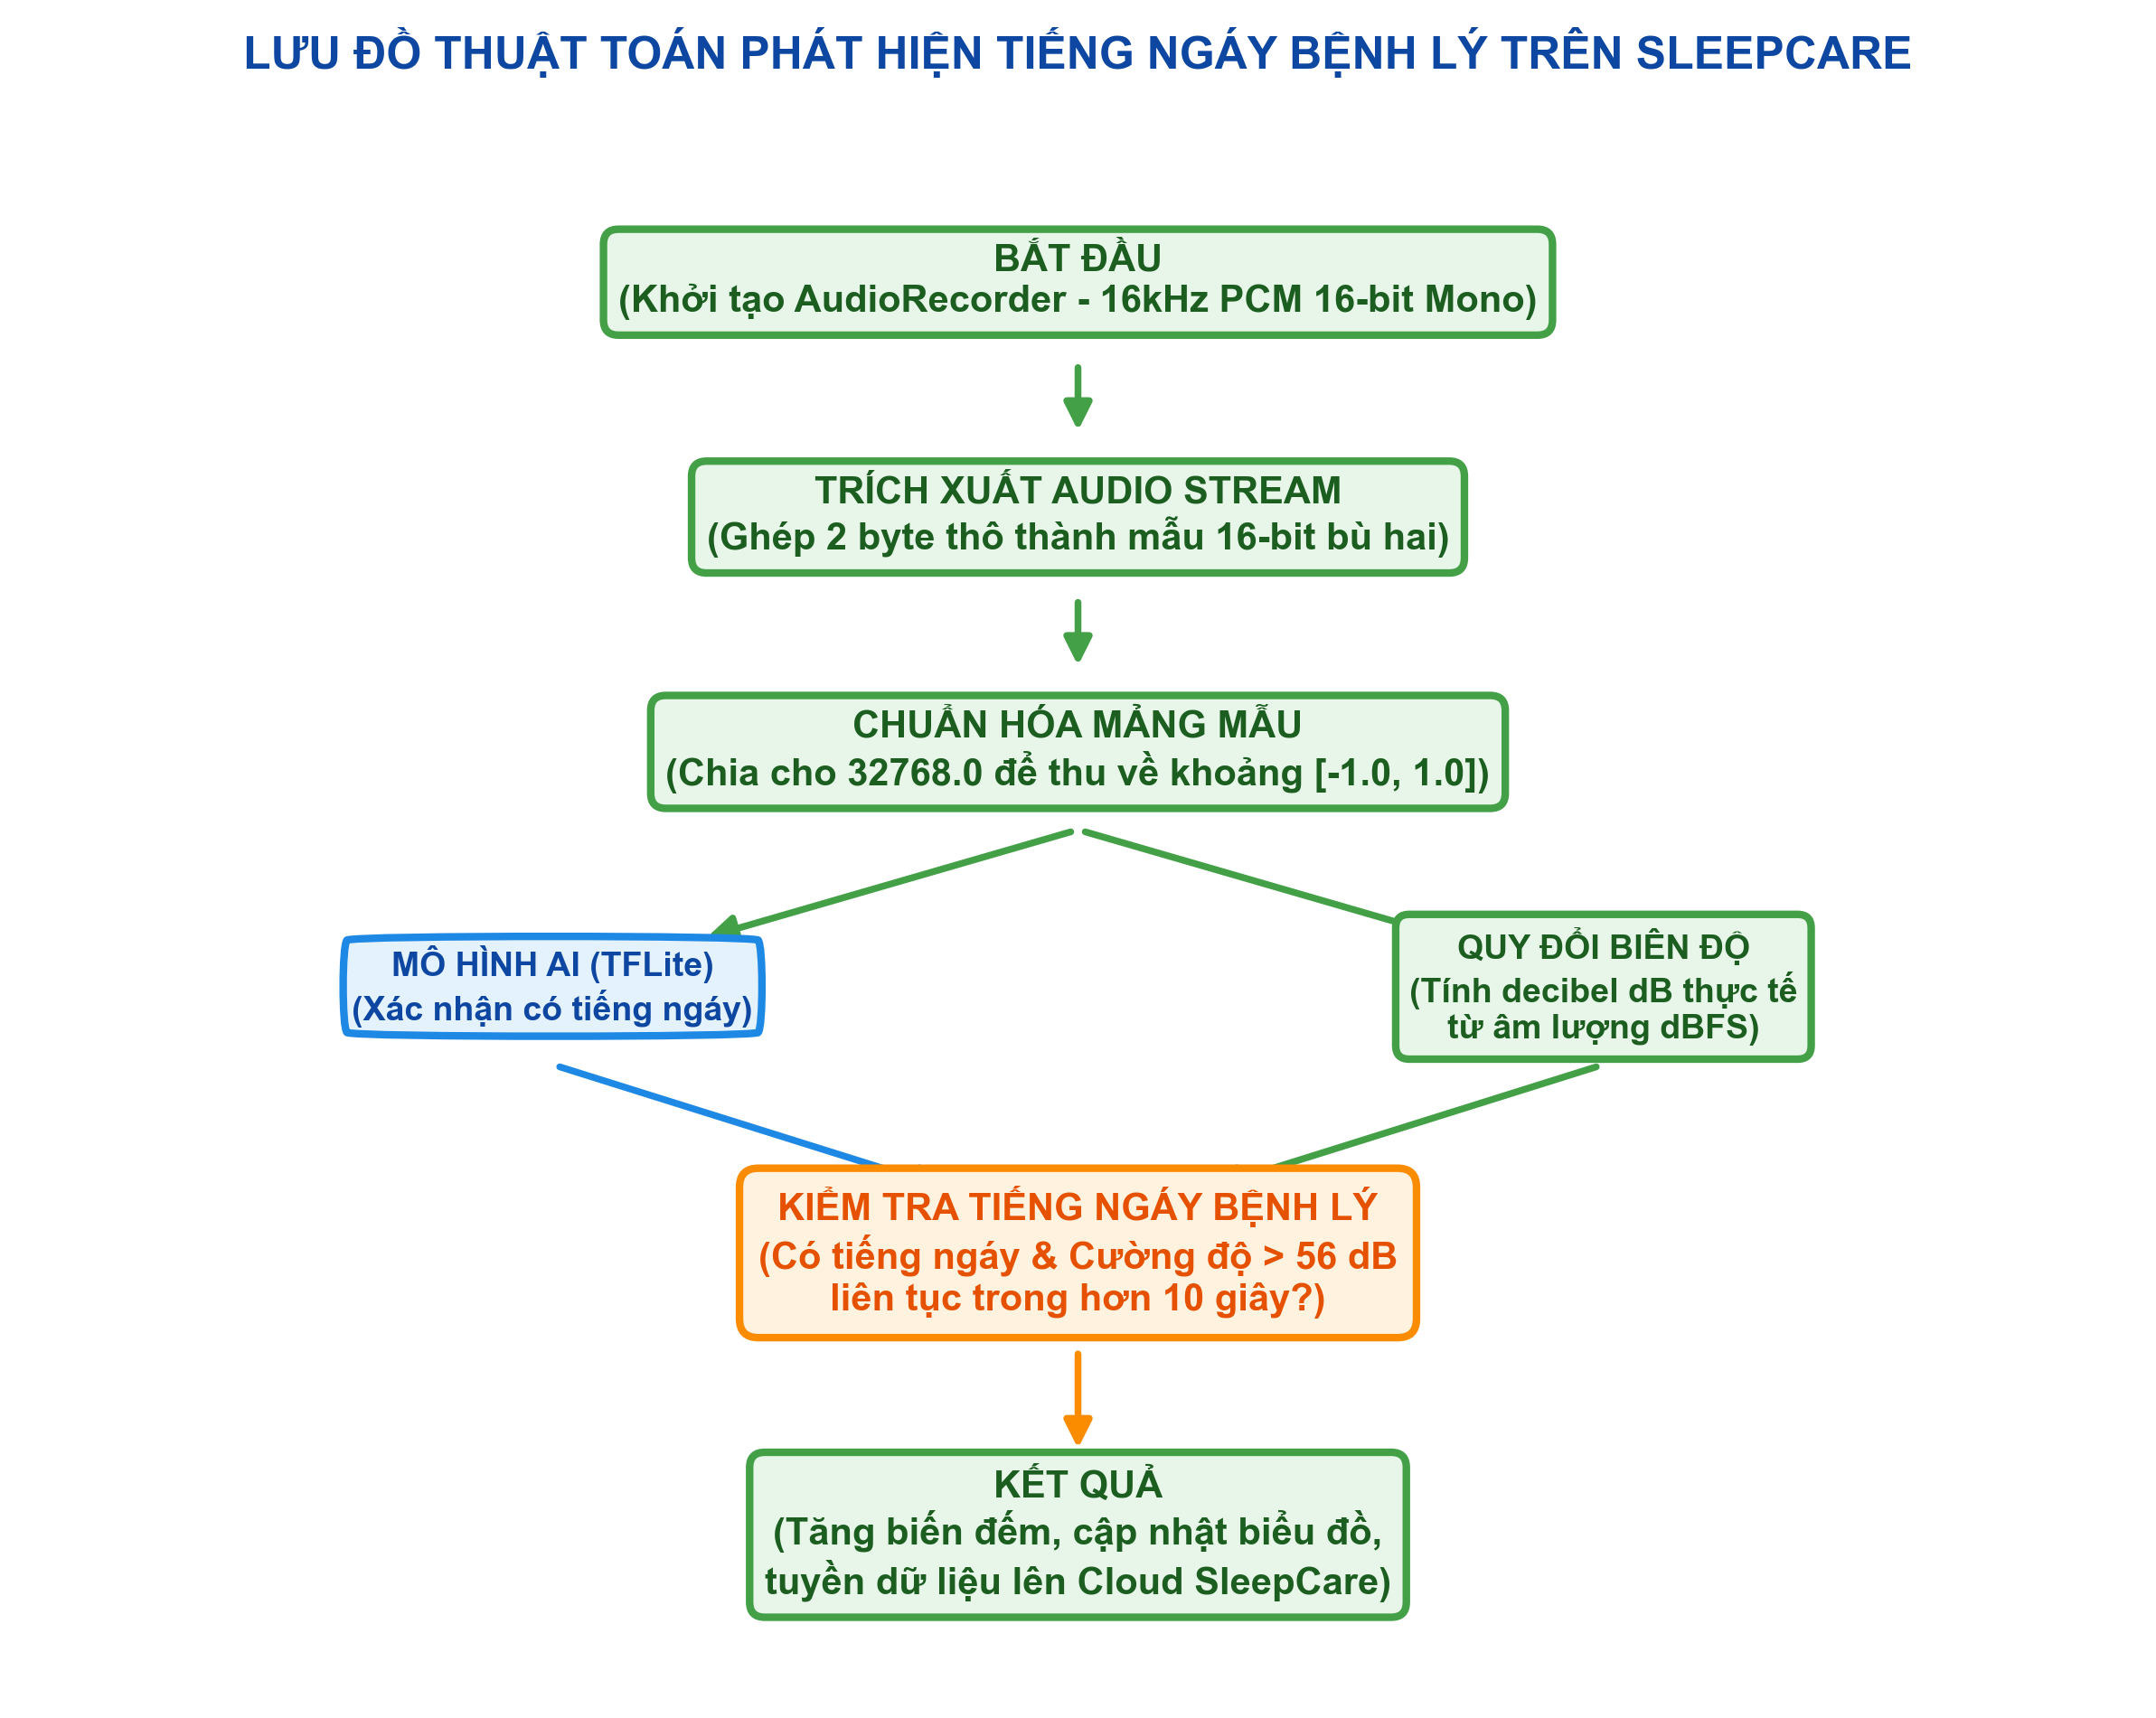
\includegraphics[width=0.7\textwidth]{snore_detection_algorithm.png}
    \caption{Lưu đồ thuật toán phát hiện tiếng ngáy bệnh lý thời gian thực từ tín hiệu ghi âm.}
    \label{fig:snore_alg}
\end{figure}

\subsubsection*{b) Thuật toán đo cường độ ánh sáng và tiếng ồn phòng ngủ}
* **Đo tiếng ồn nền:** Sử dụng microphone ghi nhận liên tục cường độ decibel ($dB$) trung bình và cực đại của phòng ngủ mỗi giây, giúp xác định xem tiếng ồn môi trường có ảnh hưởng đến pha ngủ sâu của bệnh nhân hay không (ngưỡng khuyến nghị dưới 35 dB).

\noindent * **Đo cường độ ánh sáng:**
\begin{itemize}
    \item Trên các thiết bị Android: Sử dụng trực tiếp dữ liệu từ cảm biến ánh sáng phần cứng (Ambient Light Sensor) thông qua luồng dữ liệu \texttt{LightSensor.luxStream()} để lấy giá trị Lux thực tế.
    \item Trên các thiết bị iOS hoặc Android không hỗ trợ cảm biến ánh sáng: Sử dụng camera trước để bắt luồng hình ảnh (\texttt{CameraImage stream}) ở độ phân giải thấp nhằm tiết kiệm pin. Thuật toán phân tích độ sáng trung bình $B$ của các pixel ảnh trên thang $[0, 255]$, sau đó quy đổi ra Lux bằng công thức thực nghiệm:
    \begin{equation}
        \text{Lux} = \frac{B}{255.0} \times 200.0
    \end{equation}
    Sau đó giá trị Lux được ánh xạ thành nhiệt độ màu tương đương (Kelvin) để đưa ra đánh giá về ánh sáng phòng ngủ.
\end{itemize}

\subsection{Thuật toán và công thức tính điểm các bảng hỏi lâm sàng}
Hệ thống di động SleepCare số hóa và tích hợp 11 bảng hỏi cùng chỉ số lâm sàng chuẩn y sinh để tầm soát đa chiều sức khỏe giấc ngủ, tâm thần và hô hấp của người dùng. Dưới đây mô tả chi tiết nội dung từng bảng hỏi, thang điểm của từng câu hỏi và thuật toán tính tổng điểm, phân loại rủi ro:

\subsubsection*{1. Chỉ số khối cơ thể (Body Mass Index - BMI)}
\begin{itemize}
    \item \textbf{Mục đích đo:} Đánh giá tình trạng dinh dưỡng, thừa cân và béo phì của người dùng - một trong những yếu tố rủi ro hàng đầu gây ngưng thở khi ngủ do tắc nghẽn (OSA).
    \item \textbf{Phương pháp đo:} Người dùng nhập chiều cao $H$ (cm) và cân nặng $W$ (kg).
    \item \textbf{Công thức tính toán:}
    \begin{equation}
        \text{BMI} = \frac{W}{(H/100)^2}
    \end{equation}
    \item \textbf{Phân loại rủi ro thừa cân/béo phì (Chuẩn Quốc tế):} 
    \begin{itemize}
        \item Gầy: $\text{BMI} < 18.5$
        \item Bình thường: $18.5 \le \text{BMI} < 25$
        \item Thừa cân: $25 \le \text{BMI} < 30$
        \item Béo phì: $\text{BMI} \ge 30$
    \end{itemize}
\end{itemize}

\subsubsection*{2. Bảng hỏi tầm soát ngưng thở khi ngủ STOP-BANG}
\begin{itemize}
    \item \textbf{Mục đích đo:} Tầm soát nhanh nguy cơ mắc Hội chứng ngưng thở khi ngủ do tắc nghẽn (OSA).
    \item \textbf{Bộ câu hỏi gồm 8 tiêu chí lâm sàng (Có/Không):}
    \begin{enumerate}
        \item \textbf{Ngáy:} Ông (bà) có ngáy to hơn cả lúc nói hay đến mức mà người ta có thể nghe thấy cho dù ở một phòng khác?
        \item \textbf{Mệt mỏi:} Ông (bà) có cảm thấy thường xuyên mệt mỏi hay buồn ngủ vào ban ngày không?
        \item \textbf{Quan sát:} Có ai thấy ông (bà) ngưng thở trong khi ngủ không?
        \item \textbf{Huyết áp:} Ông (bà) có đang được điều trị tăng huyết áp không?
        \item \textbf{BMI:} Chỉ số khối cơ thể BMI của ông (bà) có lớn hơn $30\text{ kg/m}^2$ không? (Hệ thống tự động tính từ thông tin nhân trắc học).
        \item \textbf{Vòng cổ:} Vòng cổ của ông (bà) có $\ge 40\text{ cm}$ không? (đo ngang trái khế).
        \item \textbf{Tuổi:} Tuổi của ông (bà) có trên 50 tuổi không?
        \item \textbf{Giới tính:} Giới tính Nam?
    \end{enumerate}
    \item \textbf{Cách tính điểm từng câu:} Câu trả lời "Có" = 1 điểm, "Không" = 0 điểm.
    \item \textbf{Thuật toán tính tổng điểm:}
    \begin{equation}
        \text{Score}_{\text{STOP-BANG}} = \sum_{i=1}^{8} X_i \quad (X_i \in \{0, 1\})
    \end{equation}
    \item \textbf{Ngưỡng phân loại rủi ro:}
    \begin{itemize}
        \item Nguy cơ cao mắc OSA: $\text{Score}_{\text{STOP-BANG}} \ge 3$
        \item Nguy cơ thấp mắc OSA: $\text{Score}_{\text{STOP-BANG}} < 3$
    \end{itemize}
\end{itemize}

\subsubsection*{3. Thang đo buồn ngủ ban ngày Epworth (ESS)}
\begin{itemize}
    \item \textbf{Mục đích đo:} Đo lường mức độ buồn ngủ ban ngày của người dùng trong các tình huống sinh hoạt thường nhật.
    \item \textbf{Bộ câu hỏi gồm 8 tình huống đánh giá:}
    \begin{enumerate}
        \item Đang ngồi đọc sách
        \item Đang xem tivi
        \item Ngồi im, không hoạt động ở nơi công cộng (rạp chiếu phim, nhà hát, trong cuộc họp)
        \item Ngồi trong ô tô (hoặc phương tiện giao thông công cộng) chạy liên tục trên một giờ không dừng
        \item Nằm nghỉ buổi chiều trong hoàn cảnh cho phép
        \item Ngồi và nói chuyện với một người nào đó
        \item Ngồi im sau một bữa ăn trưa không uống nhiều rượu
        \item Ngồi trong ô tô khi xe cần phải dừng lại vài phút (đèn đỏ, kẹt xe)
    \end{enumerate}
    \item \textbf{Cách tính điểm từng câu:} Người dùng tự chấm theo thang điểm Likert 4 mức:
    \begin{itemize}
        \item 0 điểm: Không bao giờ ngủ gật
        \item 1 điểm: Cơ may ngủ gật nhẹ
        \item 2 điểm: Cơ may ngủ gật vừa
        \item 3 điểm: Cơ may ngủ gật cao
    \end{itemize}
    \item \textbf{Thuật toán tính tổng điểm:}
    \begin{equation}
        \text{Score}_{\text{ESS}} = \sum_{i=1}^{8} S_i \quad (S_i \in [0, 3])
    \end{equation}
    \item \textbf{Ngưỡng phân loại buồn ngủ ban ngày:}
    \begin{itemize}
        \item Bình thường: $\text{Score}_{\text{ESS}} < 8$
        \item Buồn ngủ nhẹ: $8 \le \text{Score}_{\text{ESS}} \le 9$
        \item Buồn ngủ nhiều: $10 \le \text{Score}_{\text{ESS}} \le 15$
        \item Buồn ngủ quá mức: $\text{Score}_{\text{ESS}} \ge 16$
    \end{itemize}
\end{itemize}

\subsubsection*{4. Thang tự đánh giá lo âu Zung (SAS)}
\begin{itemize}
    \item \textbf{Mục đích đo:} Đánh giá mức độ nghiêm trọng của các triệu chứng rối loạn lo âu.
    \item \textbf{Bộ câu hỏi gồm 20 trạng thái cảm xúc và cơ thể:}
    \begin{enumerate}
        \item Tôi cảm thấy nóng nảy và lo âu hơn thường lệ.
        \item Tôi cảm thấy sợ vô cớ.
        \item Tôi dễ bối rối và cảm thấy hoảng sợ.
        \item Tôi thường có ác mộng.
        \item Tôi cảm thấy như bị ngã và vỡ ra từng mảnh (bủn rủn chân tay).
        \item Tôi cảm thấy mọi thứ đều tốt và không có điều gì xấu sẽ xảy ra.
        \item Tay và chân tôi lắc lư, run lên.
        \item Tôi đang khó chịu vì đau đầu, đau cổ, đau lưng.
        \item Tôi cảm thấy yếu và dễ mệt mỏi.
        \item Tôi cảm thấy bình tĩnh và có thể ngồi yên một cách dễ dàng.
        \item Tôi cảm thấy tim mình đập nhanh.
        \item Tôi đang khó chịu vì cơn hoa mắt chóng mặt.
        \item Tôi bị ngất và có lúc cảm thấy gần như thế.
        \item Tôi có thể thở ra, hít vào một cách dễ dàng.
        \item Tôi cảm thấy tê buốt, như có kiến bò ở đầu ngón tay, ngón chân.
        \item Tôi đang khó chịu vì đau dạ dày và đầy bụng.
        \item Tôi luôn cần phải đi tiểu.
        \item Bàn tay tôi thường khô và ấm.
        \item Tôi ngủ dễ dàng và luôn có một giấc ngủ tốt.
        \item Mặt tôi thường nóng và đỏ.
    \end{enumerate}
    \item \textbf{Cách tính điểm từng câu:}
    Người dùng chọn theo tần suất xuất hiện: 0 (Không hoặc hiếm khi), 1 (Đôi khi), 2 (Phần lớn thời gian), 3 (Hầu như luôn luôn).
    \begin{itemize}
        \item \textbf{Đối với 15 câu thuận} (câu 1-3, 5, 7-9, 11-13, 15-17, 20): Điểm số của câu $i$ là:
        \begin{equation}
            S_i = v_i + 1 \quad (S_i \in [1, 4])
        \end{equation}
        \item \textbf{Đối với 5 câu nghịch (đảo ngược)} (câu 6, 10, 14, 18, 19): Điểm số của câu $i$ được tính bằng cách lấy 4 trừ đi giá trị chọn:
        \begin{equation}
            S_i = 4 - v_i \quad (S_i \in [1, 4])
        \end{equation}
    \end{itemize}
    \item \textbf{Thuật toán tính tổng điểm:}
    \begin{equation}
        \text{Score}_{\text{Zung}} = \sum_{i \in \text{Thuận}} (v_i + 1) + \sum_{i \in \text{Ngược}} (4 - v_i) \quad (\text{Thang điểm từ } 20 \text{ đến } 80)
    \end{equation}
    \item \textbf{Ngưỡng phân loại lo âu:}
    \begin{itemize}
        \item Không lo âu: $\text{Score}_{\text{Zung}} < 41$
        \item Lo âu nhẹ: $41 \le \text{Score}_{\text{Zung}} \le 50$
        \item Lo âu vừa: $51 \le \text{Score}_{\text{Zung}} \le 60$
        \item Lo âu nặng: $61 \le \text{Score}_{\text{Zung}} \le 70$
        \item Lo âu rất nặng: $\text{Score}_{\text{Zung}} \ge 71$
    \end{itemize}
\end{itemize}

\subsubsection*{5. Thang đánh giá trầm cảm Hamilton (HAM-D 17 mục)}
\begin{itemize}
    \item \textbf{Mục đích đo:} Đo lường mức độ nghiêm trọng của hội chứng trầm cảm lâm sàng.
    \item \textbf{Bộ câu hỏi gồm 17 triệu chứng bệnh lý và thang điểm từng câu:}
    \begin{enumerate}
        \item \textbf{Khí sắc trầm} (Buồn bã, bi quan về tương lai, khóc lóc): 0 (Không), 1 (Nhẹ), 2 (Vừa), 3 (Nặng), 4 (Rất nặng).
        \item \textbf{Cảm giác tội lỗi} (Tự trách mình vì sai lầm hoặc tội lỗi): 0 (Không), 1 (Nhẹ), 2 (Ý nghĩ tự buộc tội), 3 (Coi bệnh là hình phạt), 4 (Ảo giác bị buộc tội).
        \item \textbf{Ý tưởng tự sát} (Cảm thấy cuộc sống vô nghĩa, có ý tưởng hoặc hành vi tự sát): 0 (Không), 1 (Cảm thấy sống vô nghĩa), 2 (Muốn chết), 3 (Có ý tưởng rõ rệt/dự định), 4 (Chuẩn bị và có hành vi).
        \item \textbf{Mất ngủ - giai đoạn đầu} (Khó đi vào giấc ngủ): 0 (Không), 1 (Thỉnh thoảng khó ngủ), 2 (Thường xuyên khó ngủ).
        \item \textbf{Mất ngủ - giai đoạn giữa} (Tỉnh giấc trong đêm, trằn trọc bồn chồn): 0 (Không), 1 (Thỉnh thoảng tỉnh giấc), 2 (Thường xuyên tỉnh giấc ban đêm).
        \item \textbf{Mất ngủ - giai đoạn cuối} (Thức dậy quá sớm và không thể ngủ lại được): 0 (Không), 1 (Thức dậy sớm nhưng ngủ lại được), 2 (Thức dậy sớm hẳn và mất ngủ hoàn toàn).
        \item \textbf{Công việc và hoạt động} (Kém hứng thú, giảm sút hiệu suất hoạt động thực tế): 0 (Không), 1 (Kém nhiệt tình, thụ động), 2 (Mất hứng thú sở thích cũ), 3 (Giảm hiệu suất công việc rõ rệt), 4 (Không thể làm việc, bỏ việc).
        \item \textbf{Chậm chạp} (Chậm chạp trong suy nghĩ, lời nói, hoạt động): 0 (Không), 1 (Chậm chạp nhẹ khi khám), 2 (Chậm chạp rõ rệt), 3 (Cực kỳ chậm chạp), 4 (Bất động sững sờ hoàn toàn).
        \item \textbf{Kích động} (Bứt rứt, bồn chồn đứng ngồi không yên): 0 (Không), 1 (Có chút bồn chồn), 2 (Vặn tay, đứng lên ngồi xuống nhiều), 3 (Cực kỳ bứt rứt, đi lại liên tục), 4 (Vò đầu bứt tai, đập phá).
        \item \textbf{Lo âu tâm lý} (Tăng lo âu, căng thẳng, cáu gắt): 0 (Không), 1 (Căng thẳng nhẹ), 2 (Lo lắng viển vông về tương lai), 3 (Thường xuyên bứt rứt sợ hãi), 4 (Cơn hoảng loạn sợ hãi cực độ).
        \item \textbf{Lo âu thể chất} (Các triệu chứng cơ thể như khó tiêu, tim đập nhanh, đau đầu, khó thở): 0 (Không), 1 (Nhẹ), 2 (Vừa), 3 (Nặng), 4 (Mất khả năng sinh hoạt vì triệu chứng).
        \item \textbf{Triệu chứng cơ thể - dạ dày và ruột} (Mất sự ngon miệng, nặng bụng, táo bón): 0 (Không), 1 (Nhẹ), 2 (Nặng).
        \item \textbf{Triệu chứng cơ thể chung} (Nặng nề tay chân, đầu, đau lưng, mệt mỏi rã rời): 0 (Không), 1 (Có biểu hiện mệt mỏi nhẹ), 2 (Cảm thấy mệt mỏi, bất lực cực độ).
        \item \textbf{Triệu chứng sinh dục} (Giảm ham muốn tình dục, rối loạn kinh nguyệt ở nữ): 0 (Không), 1 (Nhẹ), 2 (Mất ham muốn hoàn toàn).
        \item \textbf{Nghi ngờ mắc bệnh} (Lo sợ bị bệnh nặng, quá chú ý cơ thể): 0 (Không), 1 (Hơi lo lắng quá mức), 2 (Quá bận tâm về sức khỏe), 3 (Thường xuyên than vãn), 4 (Hoang tưởng nghi bệnh).
        \item \textbf{Sút cân} (Sút cân trong thời gian ngắn): 0 (Không), 1 (Sút cân nhẹ), 2 (Sút cân nhiều).
        \item \textbf{Nhận thức ý thức bệnh} (Nhận thức được mình đang mắc bệnh tâm lý): 0 (Nhận thức đầy đủ), 1 (Nhận thức một phần hoặc không rõ), 2 (Phủ nhận hoàn toàn tình trạng bệnh).
    \end{enumerate}
    \item \textbf{Cách tính điểm từng câu:} Hệ thống tự động lấy chỉ số index của phương án người dùng đã lựa chọn (chạy từ 0 đến điểm tối đa của câu hỏi đó).
    \item \textbf{Thuật toán tính tổng điểm:}
    \begin{equation}
        \text{Score}_{\text{Hamilton}} = \sum_{i=1}^{17} \text{index}_i \quad (\text{Thang điểm từ } 0 \text{ đến } 52)
    \end{equation}
    \item \textbf{Ngưỡng phân loại trầm cảm:}
    \begin{itemize}
        \item Không trầm cảm: $\text{Score}_{\text{Hamilton}} < 8$
        \item Trầm cảm nhẹ: $8 \le \text{Score}_{\text{Hamilton}} \le 13$
        \item Trầm cảm trung bình: $14 \le \text{Score}_{\text{Hamilton}} \le 18$
        \item Trầm cảm nặng: $19 \le \text{Score}_{\text{Hamilton}} \le 22$
        \item Trầm cảm rất nặng: $\text{Score}_{\text{Hamilton}} \ge 23$
    \end{itemize}
\end{itemize}

\subsubsection*{6. Chỉ số Chất lượng Giấc ngủ Pittsburgh (PSQI)}
\begin{itemize}
    \item \textbf{Mục đích đo:} Đánh giá chất lượng và các rối loạn giấc ngủ của cá nhân trong vòng 1 tháng qua.
    \item \textbf{Thuật toán tính điểm 7 thành phần (mỗi thành phần chạy từ 0 đến 3 điểm):}
    \begin{itemize}
        \item \textbf{Thành phần 1: Chất lượng giấc ngủ chủ quan.} Trực tiếp lấy từ điểm câu số 6 (chất lượng giấc ngủ tự nhận đánh giá: Rất tốt = 0, Khá tốt = 1, Khá kém = 2, Rất kém = 3).
        \item \textbf{Thành phần 2: Độ trễ giấc ngủ (Sleep Latency).} Tính tổng hợp từ số phút để đi vào giấc ngủ (Câu 2) và tần suất không thể đi vào giấc ngủ trong vòng 30 phút (Câu 5a). Quy đổi tổng điểm ra thang 0-3 điểm.
        \item \textbf{Thành phần 3: Thời lượng giấc ngủ (Sleep Duration).} Dựa trên số giờ ngủ thực tế ban đêm (Câu 4): $\ge 7\text{ giờ} = 0$ điểm, $6 \le \text{giờ} < 7 = 1$ điểm, $5 \le \text{giờ} < 6 = 2$ điểm, $< 5\text{ giờ} = 3$ điểm.
        \item \textbf{Thành phần 4: Hiệu quả giấc ngủ thực tế (Habitual Sleep Efficiency).} 
        \begin{equation}
            \text{Hiệu quả} = \frac{\text{Thời lượng giấc ngủ thực tế (Câu 4)}}{\text{Thời gian nằm trên giường (Giờ thức giấc Câu 3 - Giờ đi ngủ Câu 1)}} \times 100\%
        \end{equation}
        Quy đổi: $\ge 84\% = 0$ điểm, $74-83\% = 1$ điểm, $65-73\% = 2$ điểm, $< 65\% = 3$ điểm.
        \item \textbf{Thành phần 5: Rối loạn giấc ngủ (Sleep Disturbances).} Tổng điểm tần suất của các sự kiện ban đêm (thức giấc giữa đêm, đi vệ sinh, ho ngáy to, nóng quá, lạnh quá, ác mộng, đau đớn...). Tổng điểm quy đổi ra thang 0-3 điểm.
        \item \textbf{Thành phần 6: Sử dụng thuốc ngủ (Use of Sleep Medication).} Tần suất sử dụng thuốc ngủ kê đơn hoặc không kê đơn (Câu 7): Không dùng = 0, $<1$ lần/tuần = 1, $1-2$ lần/tuần = 2, $\ge 3$ lần/tuần = 3.
        \item \textbf{Thành phần 7: Rối loạn chức năng ban ngày (Daytime Dysfunction).} Cộng điểm của tần suất buồn ngủ khi lái xe/ăn uống/hoạt động (Câu 8) và mức độ thiếu nhiệt tình hoàn thành công việc (Câu 9). Quy đổi tổng ra thang 0-3 điểm.
    \end{itemize}
    \item \textbf{Thuật toán tính tổng điểm PSQI:}
    \begin{equation}
        \text{Score}_{\text{PSQI}} = \sum_{j=1}^{7} C_j \quad (\text{Thang điểm từ } 0 \text{ đến } 21)
    \end{equation}
    \item \textbf{Ngưỡng phân loại chất lượng giấc ngủ:}
    \begin{itemize}
        \item Chất lượng giấc ngủ tốt: $\text{Score}_{\text{PSQI}} < 5$
        \item Chất lượng giấc ngủ trung bình: $5 \le \text{Score}_{\text{PSQI}} \le 9$
        \item Chất lượng giấc ngủ kém: $\text{Score}_{\text{PSQI}} \ge 10$
    \end{itemize}
\end{itemize}

\subsubsection*{7. Bộ câu hỏi giấc ngủ trẻ em (PSQ)}
\begin{itemize}
    \item \textbf{Mục đích đo:} Sàng lọc chứng rối loạn thở khi ngủ (Sleep-Disordered Breathing - SDB) ở trẻ em từ 2 đến 18 tuổi.
    \item \textbf{Bộ câu hỏi gồm 22 câu hỏi về thói quen của trẻ (Có/Không/Không biết):}
    \begin{enumerate}
        \item Con ông (bà) có ngủ ngáy hơn 50\% thời gian ngủ không?
        \item Con ông (bà) có luôn ngáy không?
        \item Con ông (bà) có ngáy to không?
        \item Trong khi ngủ, con ông (bà) có thở nặng nhọc hay thở ồn ào không?
        \item Trong khi ngủ, con ông (bà) có khó thở hay gắng sức để thở không?
        \item Có bao giờ ông (bà) nhận thấy con mình ngưng thở trong đêm không?
        \item Ban ngày, trẻ có xu hướng thở bằng miệng không?
        \item Trẻ có thức dậy với cảm giác khô miệng vào buổi sáng không?
        \item Thỉnh thoảng trẻ có đái dầm không?
        \item Trẻ có thấy mệt mỏi khi thức dậy vào buổi sáng không?
        \item Trẻ có buồn ngủ vào ban ngày không?
        \item Có giáo viên hay người chăm sóc nào nhận xét trẻ buồn ngủ ban ngày không?
        \item Trẻ có khó thức dậy vào buổi sáng không?
        \item Từ khi sinh ra, con ông (bà) có từng bị chậm phát triển thể chất không?
        \item Trẻ có bị đau đầu khi thức dậy vào buổi sáng không?
        \item Con ông (bà) có bị thừa cân không?
        \item Trẻ thường có vẻ như không nghe khi người khác nói trực tiếp với trẻ?
        \item Trẻ thường gặp khó khăn trong việc tổ chức công việc và hoạt động?
        \item Trẻ có dễ bị xao nhãng bởi các kích thích bên ngoài không?
        \item Trẻ có thường cựa quậy tay chân hoặc đứng ngồi không yên không?
        \item Trẻ có hay ngắt lời hoặc chen ngang vào việc của người khác không?
        \item Con ông (bà) có thường 'quá hiếu động' hay thường 'hay nói quá nhiều'?
    \end{enumerate}
    \item \textbf{Cách tính điểm từng câu:} Câu trả lời "Có" = 1 điểm, "Không" = 0 điểm. Câu trả lời "Không biết" được loại khỏi mẫu thống kê.
    \item \textbf{Thuật toán tính toán chỉ số:}
    Hệ thống tính tổng số câu trả lời dương tính $Y$ (Có) và số câu trả lời âm tính $N$ (Không).
    \begin{equation}
        \text{Ratio} = \frac{Y}{Y + N}
    \end{equation}
    \item \textbf{Ngưỡng phân loại kết quả:}
    \begin{itemize}
        \item Dương tính (Nguy cơ cao bị rối loạn thở khi ngủ): $\text{Ratio} > 0.33$ (tương đương với điều kiện toán học $Y > N/2.0$).
        \item Âm tính: $\text{Ratio} \le 0.33$.
    \end{itemize}
\end{itemize}

\subsubsection*{8. Chỉ số độ nghiêm trọng của mất ngủ (ISI)}
\begin{itemize}
    \item \textbf{Mục đích đo:} Đánh giá cảm nhận chủ quan về mức độ nghiêm trọng và tác động của chứng mất ngủ.
    \item \textbf{Bộ câu hỏi gồm 7 mục khảo sát tự đánh giá:}
    \begin{enumerate}
        \item Mức độ nghiêm trọng của khó khăn khi đi vào giấc ngủ.
        \item Mức độ nghiêm trọng của khó khăn khi duy trì giấc ngủ (thức giấc ban đêm).
        \item Mức độ nghiêm trọng của việc thức dậy quá sớm vào buổi sáng.
        \item Mức độ hài lòng/không hài lòng với giấc ngủ hiện tại của bản thân.
        \item Mức độ ảnh hưởng của rối loạn giấc ngủ đến hoạt động ban ngày (mệt mỏi, hiệu suất, tập trung).
        \item Mức độ dễ nhận thấy của chứng mất ngủ đối với người khác xung quanh.
        \item Mức độ lo lắng, buồn phiền gây ra bởi tình trạng mất ngủ hiện tại.
    \end{enumerate}
    \item \textbf{Cách tính điểm từng câu:} Người dùng tự chọn từ 0 đến 4 điểm (0: Không có/Rất hài lòng, 1: Nhẹ, 2: Vừa phải, 3: Nặng, 4: Rất nặng/Rất không hài lòng).
    \item \textbf{Thuật toán tính tổng điểm:}
    \begin{equation}
        \text{Score}_{\text{ISI}} = \sum_{i=1}^{7} S_i \quad (S_i \in [0, 4])
    \end{equation}
    \item \textbf{Ngưỡng phân loại độ nghiêm trọng của mất ngủ:}
    \begin{itemize}
        \item Không có mất ngủ lâm sàng: $\text{Score}_{\text{ISI}} < 8$
        \item Mất ngủ nhẹ: $8 \le \text{Score}_{\text{ISI}} \le 14$
        \item Mất ngủ trung bình (lâm sàng): $15 \le \text{Score}_{\text{ISI}} \le 21$
        \item Mất ngủ nặng (lâm sàng): $\text{Score}_{\text{ISI}} \ge 22$
    \end{itemize}
\end{itemize}

\subsubsection*{9. Thang đánh giá mệt mỏi Pichot}
\begin{itemize}
    \item \textbf{Mục đích đo:} Đo lường tình trạng kiệt sức và mệt mỏi bệnh lý ban ngày của người dùng.
    \item \textbf{Bộ câu hỏi gồm 8 trạng thái mệt mỏi:}
    \begin{enumerate}
        \item Tôi cảm thấy kiệt sức, yếu sức lực.
        \item Tôi thấy mệt mỏi kéo dài suốt cả ngày.
        \item Tôi cảm thấy mình hoàn toàn thiếu hụt năng lượng.
        \item Tình trạng mệt mỏi tăng lên nhanh chóng sau khi gắng sức.
        \item Tôi luôn cảm thấy buồn ngủ vào ban ngày.
        \item Tôi gặp khó khăn lớn khi tập trung do cảm thấy mệt mỏi.
        \item Sự mệt mỏi làm giảm rõ rệt các hoạt động thể chất hàng ngày.
        \item Tôi luôn cảm thấy cơ thể uể oải, trì trệ.
    \end{enumerate}
    \item \textbf{Cách tính điểm từng câu:} Likert 5 mức: 0 (Không có) đến 4 (Rất nhiều).
    \item \textbf{Thuật toán tính tổng điểm:}
    \begin{equation}
        \text{Score}_{\text{Pichot-Fatigue}} = \sum_{i=1}^{8} S_i \quad (\text{Thang điểm từ } 0 \text{ đến } 32)
    \end{equation}
    \item \textbf{Phân loại:} Bình thường khi $\text{Score}_{\text{Pichot-Fatigue}} \le 22$ điểm; có biểu hiện mệt mỏi bệnh lý khi điểm số $> 22$ điểm.
\end{itemize}

\subsubsection*{10. Thang đánh giá trầm cảm Pichot QD}
\begin{itemize}
    \item \textbf{Mục đích đo:} Sàng lọc nhanh các biểu hiện nghi ngờ trầm cảm.
    \item \textbf{Bộ câu hỏi gồm 13 câu hỏi nhị phân (Có/Không):}
    \begin{enumerate}
        \item Tôi luôn cảm thấy buồn bã, chán nản.
        \item Tôi không còn tìm thấy hứng thú với các sở thích cũ của mình.
        \item Tôi cảm thấy bi quan và lo lắng về tương lai phía trước.
        \item Tôi rất hay khóc hoặc có cảm giác muốn khóc.
        \item Tôi luôn tự cảm thấy mình vô dụng và kém cỏi.
        \item Tôi thấy rất khó khăn khi đưa ra các quyết định thường ngày.
        \item Tôi cảm thấy thường xuyên lo âu, bứt rứt trong lòng.
        \item Tôi gặp khó khăn lớn trong việc đi vào giấc ngủ và ngủ sâu.
        \item Tôi cảm thấy ăn không ngon miệng, sụt cân.
        \item Tôi luôn cảm thấy mệt mỏi rã rời, mất hoàn toàn sức sống.
        \item Tôi có cảm giác mình đang trở thành gánh nặng cho mọi người.
        \item Thỉnh thoảng tôi có ý nghĩ muốn tự giải thoát cho bản thân.
        \item Tôi thấy cuộc sống này không còn gì ý nghĩa nữa.
    \end{enumerate}
    \item \textbf{Cách tính điểm:} Câu trả lời "Có" = 1 điểm, "Không" = 0 điểm.
    \item \textbf{Thuật toán tính tổng điểm:}
    \begin{equation}
        \text{Score}_{\text{Pichot-QD}} = \sum_{i=1}^{13} X_i \quad (X_i \in \{0, 1\})
    \end{equation}
    \item \textbf{Phân loại:} Bình thường khi điểm số $\le 7$ điểm; nghi ngờ có trầm cảm bệnh lý khi điểm số $> 7$ điểm.
\end{itemize}

\subsubsection*{11. Thang trầm cảm cho người cao tuổi (GDS-15)}
\begin{itemize}
    \item \textbf{Mục đích đo:} Đo lường và tầm soát chứng trầm cảm chuyên biệt cho đối tượng người cao tuổi.
    \item \textbf{Bộ câu hỏi gồm 15 câu hỏi nhị phân (Có/Không):}
    \begin{enumerate}
        \item Ông/bànhìn chung có hài lòng với cuộc sống của mình không?
        \item Ông/bà có từ bỏ nhiều hoạt động và sở thích thường ngày của mình không?
        \item Ông/bà có cảm thấy cuộc sống hiện tại của mình trống rỗng không?
        \item Ông/bà có thường xuyên cảm thấy buồn chán không?
        \item Ông/bà có hầu như luôn ở trong trạng thái tinh thần vui vẻ không?
        \item Ông/bà có lo sợ rằng điều gì đó tồi tệ sẽ xảy ra với mình không?
        \item Ông/bà có thường xuyên cảm thấy hạnh phúc không?
        \item Ông/bà có thường cảm thấy bất lực không?
        \item Ông/bà có thích ở nhà hơn là đi ra ngoài và làm những việc mới không?
        \item Ông/bà có nghĩ mình gặp nhiều vấn đề về trí nhớ hơn những người khác không?
        \item Ông/bà có nghĩ rằng thật tuyệt vời khi được sống đến lúc này không?
        \item Ông/bà có cảm thấy mình khá vô dụng ở trạng thái hiện tại không?
        \item Ông/bà có cảm thấy mình luôn tràn đầy năng lượng không?
        \item Ông/bà có cảm thấy hoàn cảnh sống của mình là vô vọng không?
        \item Ông/bà có nghĩ rằng hầu hết mọi người đều tốt số/tốt đẹp hơn mình không?
    \end{enumerate}
    \item \textbf{Cách tính điểm từng câu:}
    \begin{itemize}
        \item \textbf{Đối với 10 câu thuận} (câu 2, 3, 4, 6, 8, 9, 10, 12, 14, 15): Điểm cộng 1 nếu trả lời "Có".
        \item \textbf{Đối với 5 câu nghịch (đảo ngược)} (câu 1, 5, 7, 11, 13): Điểm cộng 1 nếu trả lời "Không".
    \end{itemize}
    \item \textbf{Thuật toán tính tổng điểm:}
    \begin{equation}
        \text{Score}_{\text{GDS-15}} = \sum_{i \in \text{Thuận}} I(X_i = \text{"Có"}) + \sum_{i \in \text{Ngược}} I(X_i = \text{"Không"}) \quad (\text{Thang điểm từ } 0 \text{ đến } 15)
    \end{equation}
    \item \textbf{Ngưỡng phân loại trầm cảm người cao tuổi:}
    \begin{itemize}
        \item Trạng thái bình thường: $0 \le \text{Score}_{\text{GDS-15}} \le 4$
        \item Trầm cảm nhẹ: $5 \le \text{Score}_{\text{GDS-15}} \le 9$
        \item Trầm cảm nặng: $\text{Score}_{\text{GDS-15}} \ge 10$
    \end{itemize}
\end{itemize}

\subsection{Tích hợp quy trình tầm soát lâm sàng chuẩn hóa}
Ứng dụng di động SleepCare tích hợp lưu đồ tầm soát khoa học gồm 3 bước liên tiếp:
\begin{enumerate}
    \item \textbf{Bước 1: Bảng câu hỏi chung và Chỉ số khối cơ thể (BMI):} Ghi nhận tuổi, giới tính, chiều cao, cân nặng để tính chỉ số BMI, huyết áp và vòng cổ của bệnh nhân.
    \item \textbf{Bước 2: Thang đo Epworth (ESS):} Khảo sát mức độ buồn ngủ ban ngày trong 8 tình huống thường gặp với mức điểm từ 0 (không bao giờ buồn ngủ) đến 3 (buồn ngủ cao). Tổng điểm lớn hơn 10 cảnh báo tình trạng buồn ngủ ban ngày bệnh lý.
    \item \textbf{Bước 3: Bảng câu hỏi STOP-BANG:} Trả lời Có/Không cho 8 tiêu chí rủi ro lâm sàng (Ngáy to, Mệt mỏi ban ngày, Ngừng thở khi ngủ được quan sát, Huyết áp cao, BMI > 35, Tuổi > 50, Vòng cổ lớn, Giới tính nam).
\end{enumerate}
Kết quả được tính toán tổng hợp từ số câu trả lời dương tính và đưa ra mức cảnh báo rủi ro mắc hội chứng ngưng thở khi ngủ (OSA):
\begin{itemize}
    \item \textbf{Rủi ro thấp:} Tổng điểm kết hợp dưới 15. Khuyến nghị duy trì thói quen vệ sinh giấc ngủ tốt.
    \item \textbf{Rủi ro trung bình:} Tổng điểm kết hợp từ 15 đến 20. Khuyến nghị người dùng thực hiện theo dõi tiếng ngáy bằng công cụ Snore Detection trên app.
    \item \textbf{Rủi ro cao:} Tổng điểm kết hợp trên 20. Cảnh báo nguy cơ cao mắc OSA, ứng dụng tự động hiển thị danh sách các phòng khám chuyên khoa liên kết của VSSM và hướng dẫn bệnh nhân đăng ký dịch vụ đo đa ký giấc ngủ tại nhà (PSG) để chẩn đoán xác định.
\end{itemize}

\begin{figure}[h!]
    \centering
    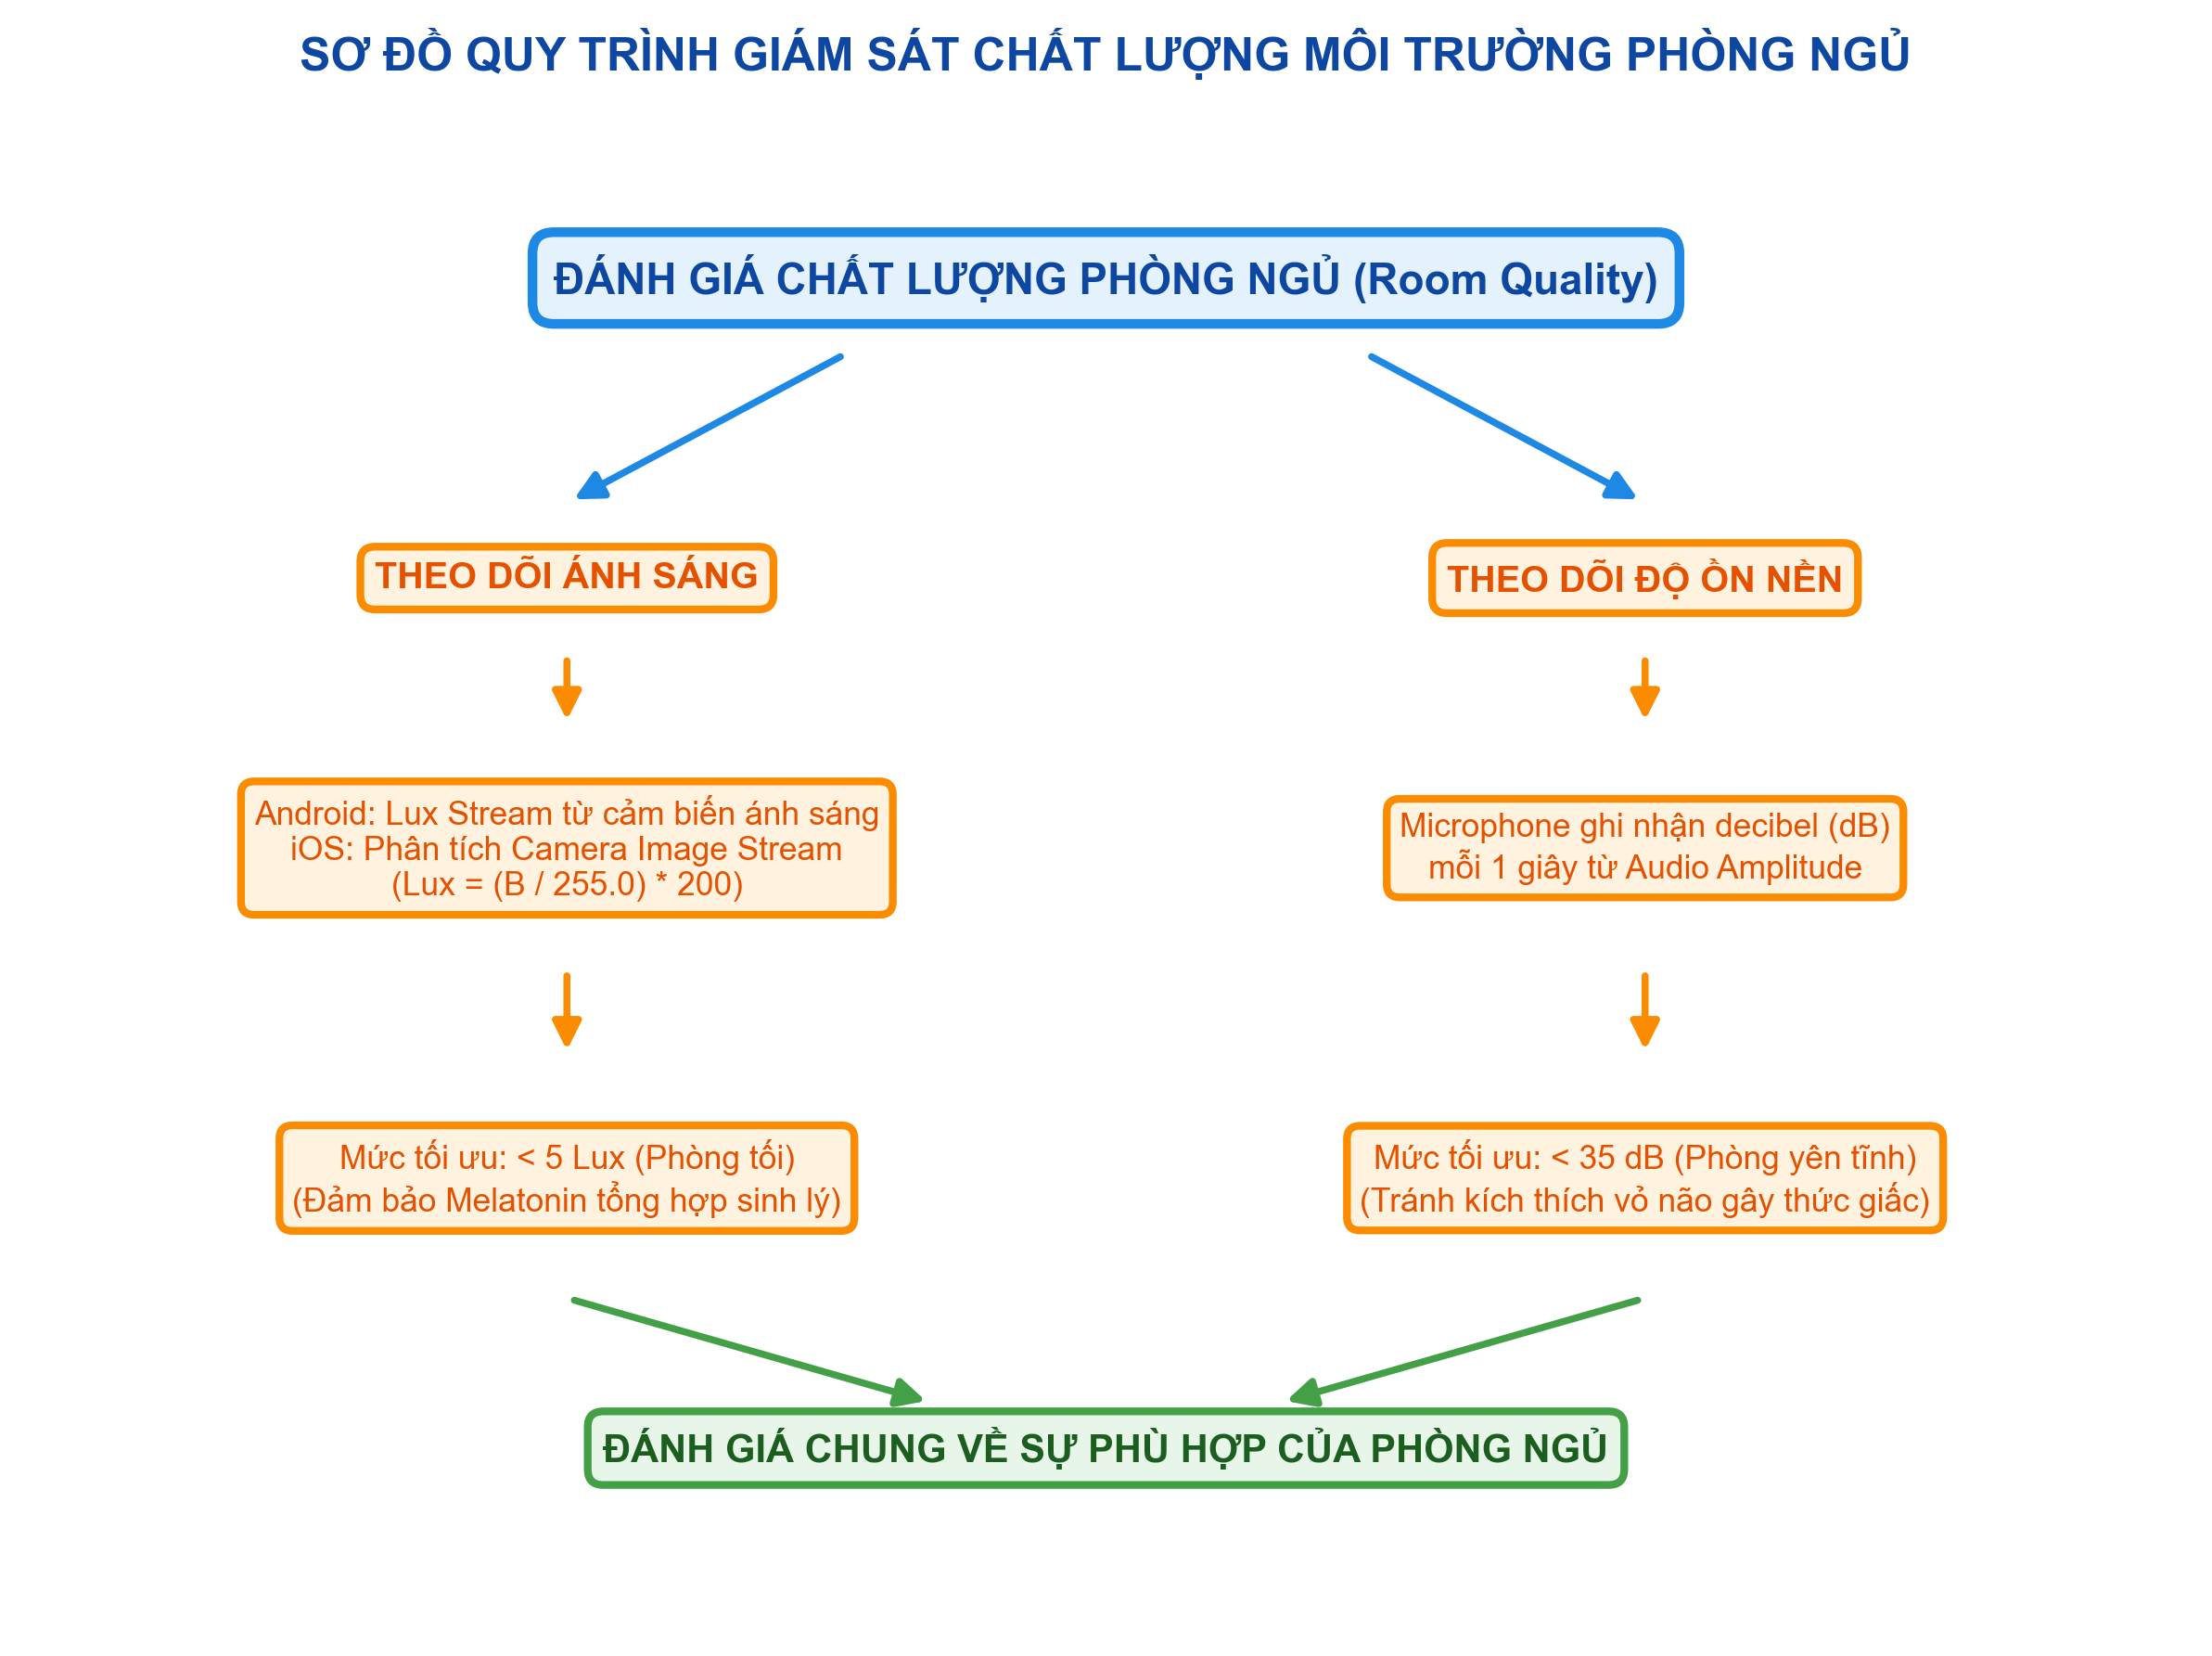
\includegraphics[width=0.7\textwidth]{room_quality_algorithm.png}
    \caption{Sơ đồ thuật toán và quy trình đo lường chất lượng phòng ngủ thông qua các cảm biến.}
    \label{fig:room_quality}
\end{figure}

\begin{figure}[h!]
    \centering
    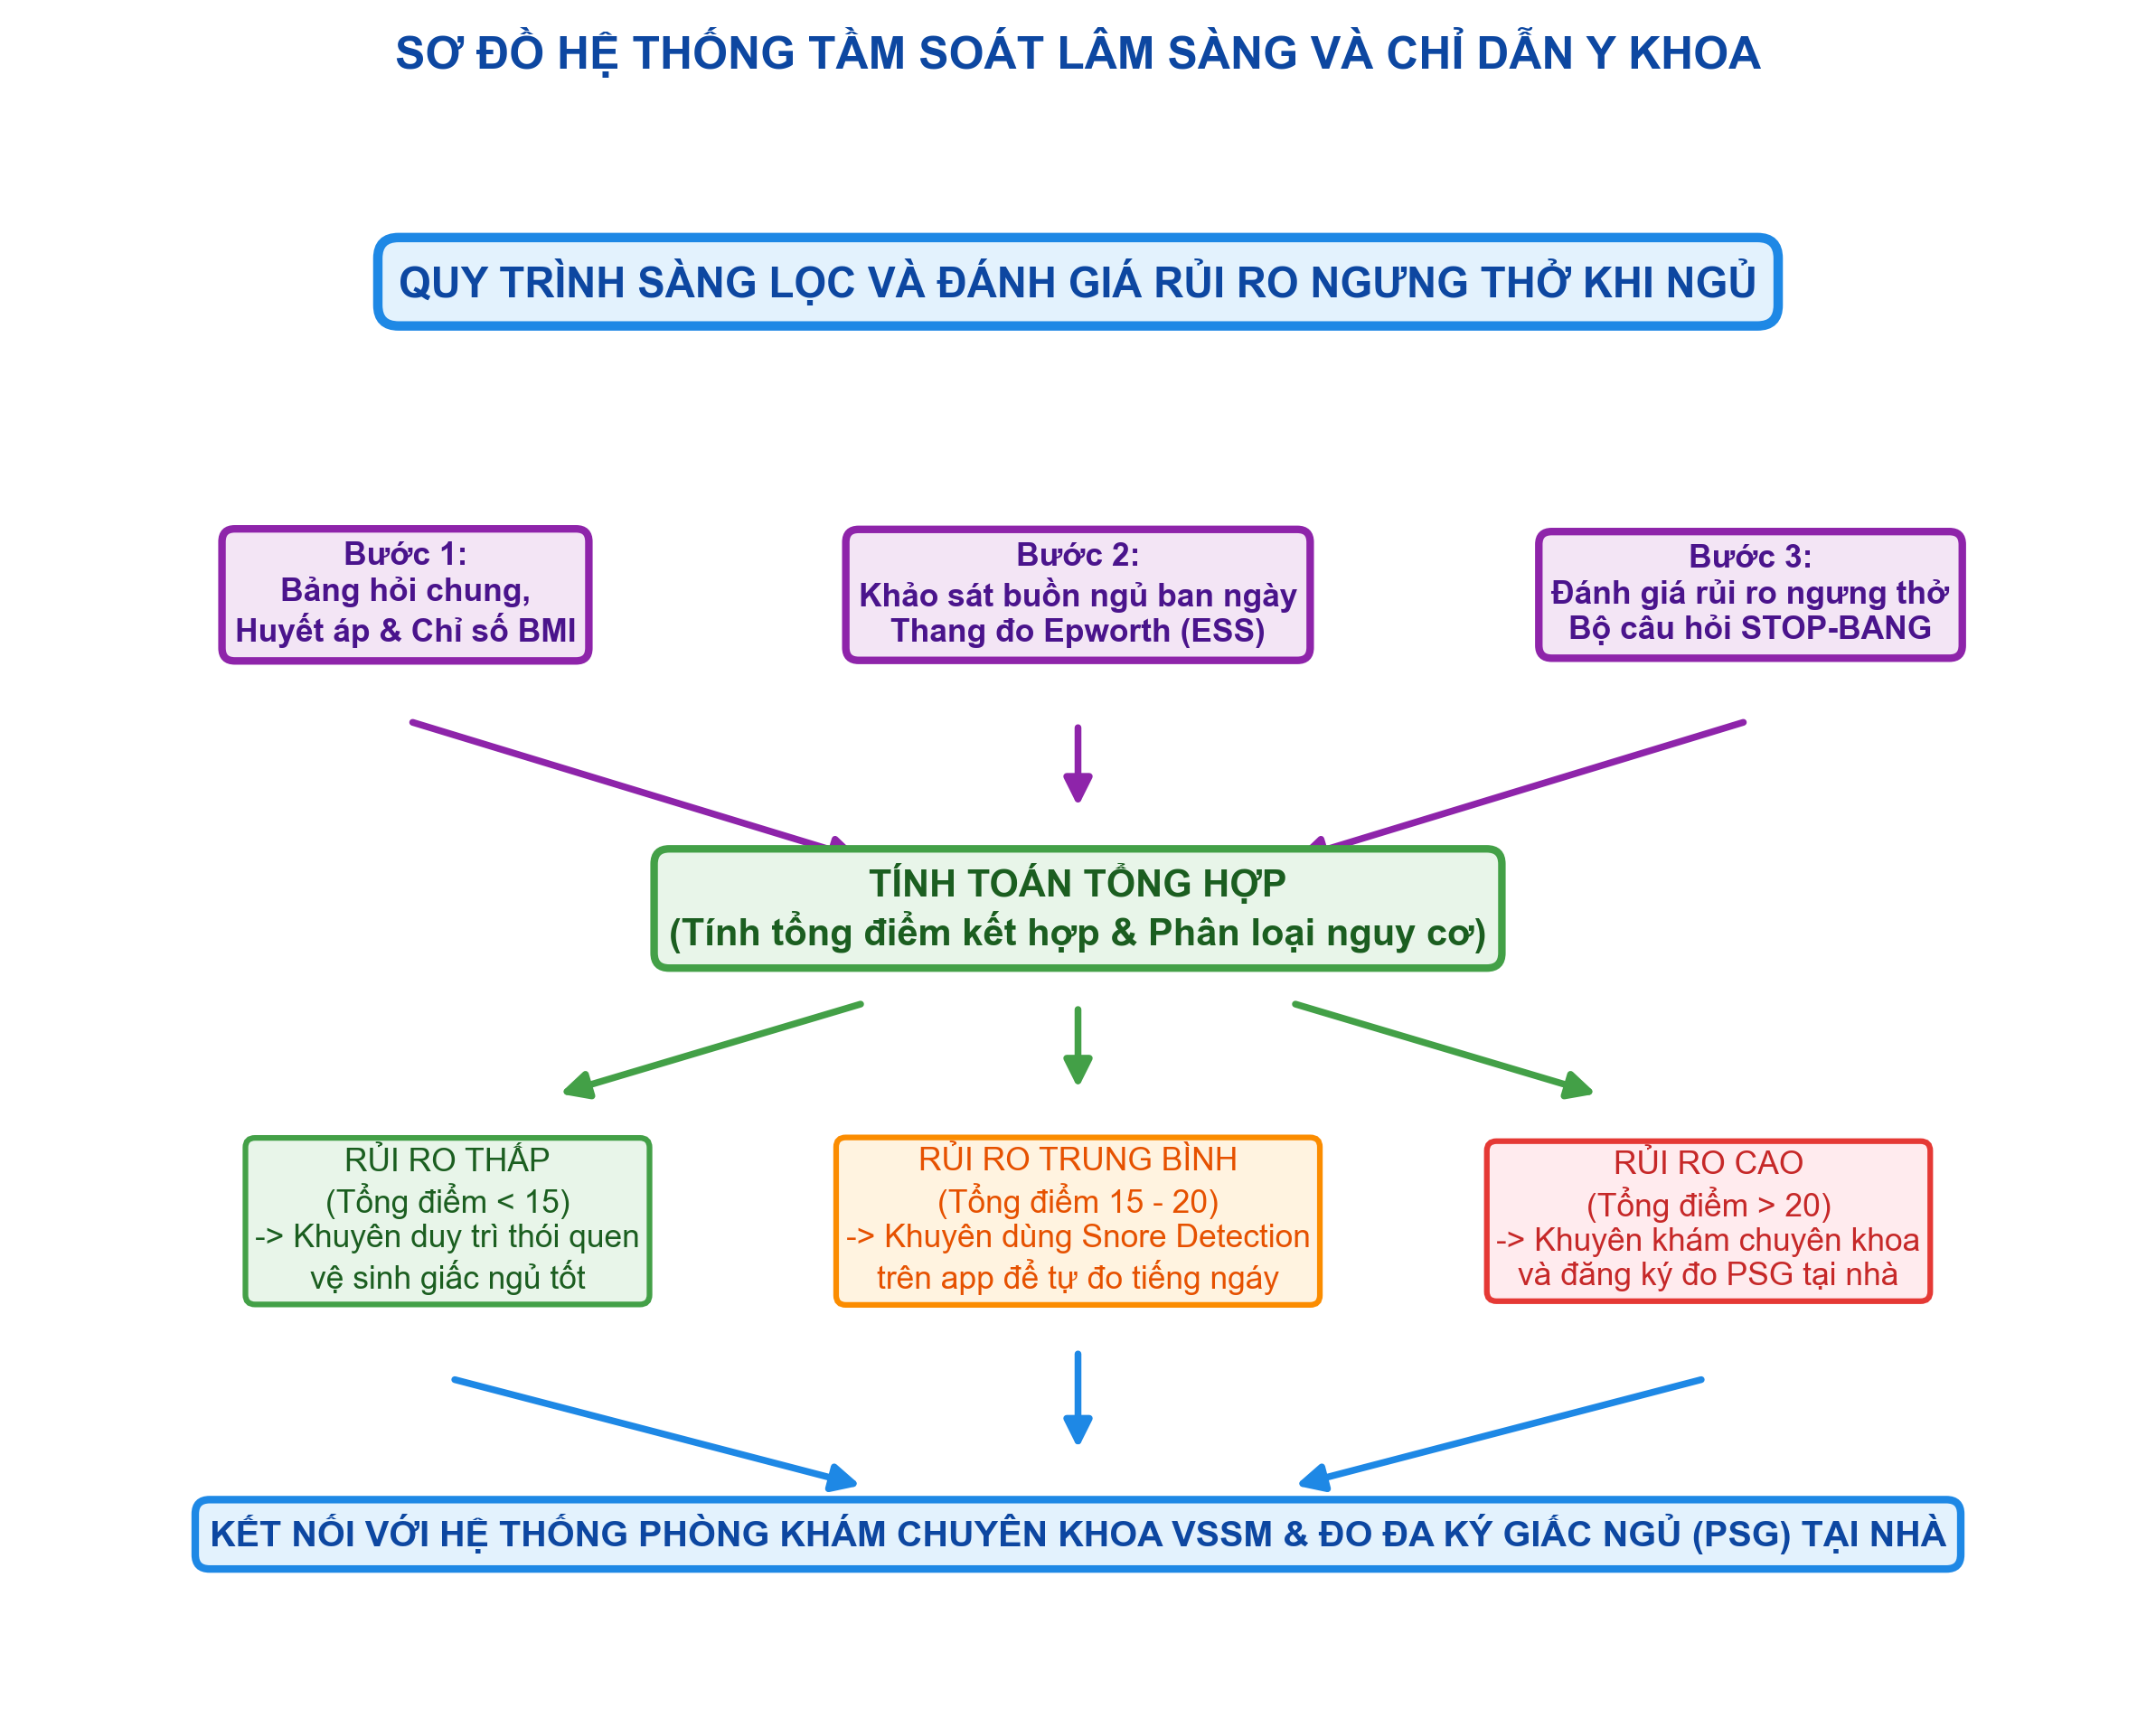
\includegraphics[width=0.7\textwidth]{screening_risk_model.png}
    \caption{Mô hình quy trình đánh giá rủi ro ngưng thở khi ngủ và kết nối y tế lâm sàng.}
    \label{fig:screening}
\end{figure}

\begin{figure}[h!]
    \centering
    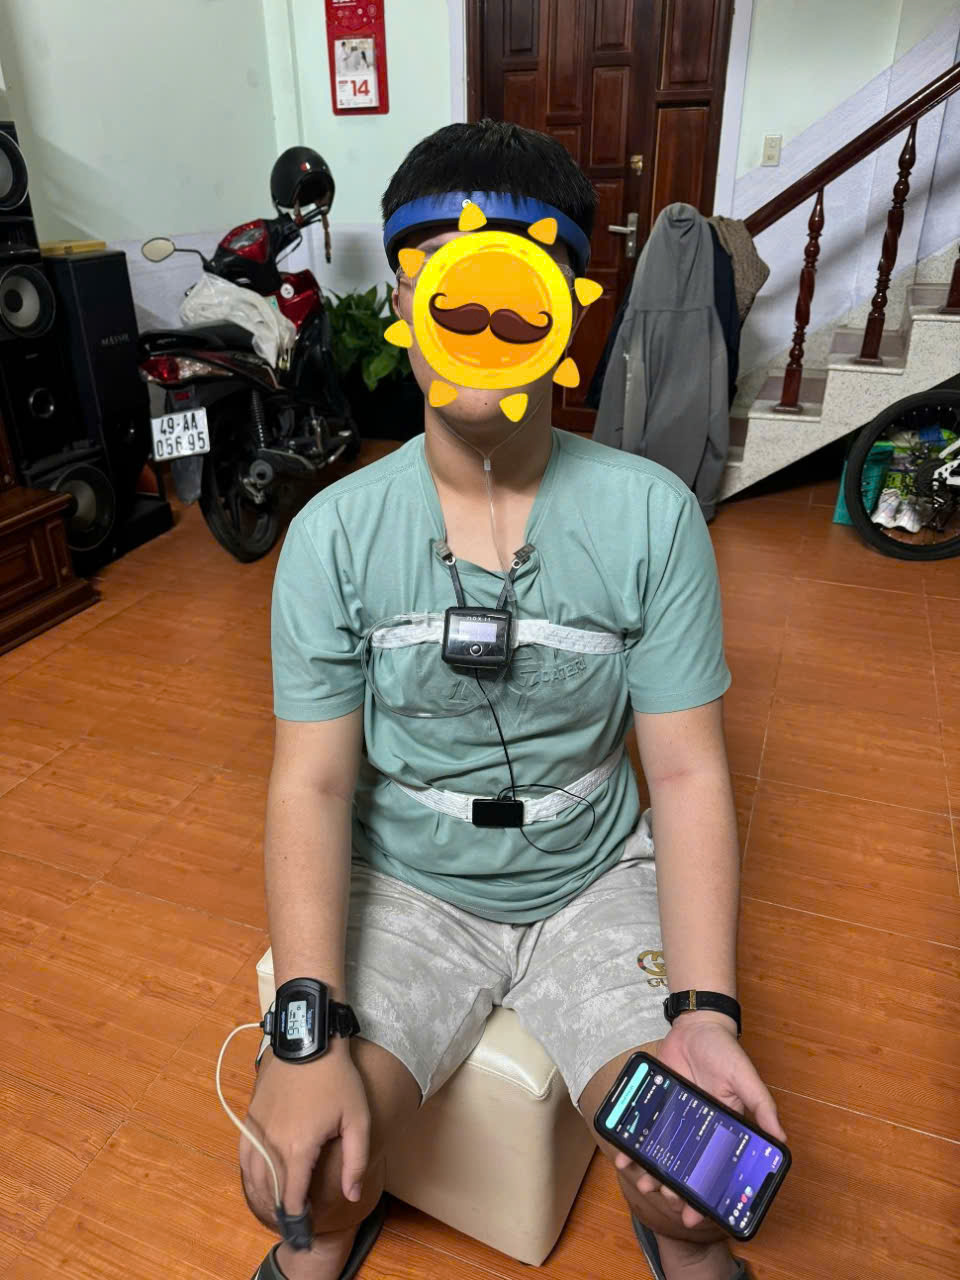
\includegraphics[width=0.5\textwidth]{doPSGTainha.jpg}
    \caption{Dịch vụ đo đa ký giấc ngủ tại nhà (PSG) liên kết giữa SleepCare và các cơ sở y tế đối tác của Hội Y học Giấc ngủ Việt Nam.}
    \label{fig:psg}
\end{figure}

% --- Section VI ---
\section{\textcolor{navy}{VI. HIỆU QUẢ ĐẠT ĐƯỢC VÀ ĐỊNH HƯỚNG PHÁT TRIỂN}}

\subsection{Hiệu quả kỹ thuật và kinh tế:}
\begin{itemize}
    \item \textbf{Không phát sinh chi phí phần cứng:} Tận dụng tối đa các cảm biến hiện có trên điện thoại di động của người dùng, giúp hàng triệu người dân có thể tự tầm soát OSA miễn phí tại nhà.
    \item \textbf{Tính chuẩn hóa lâm sàng cao:} Khác biệt hoàn toàn với các app thương mại thông thường, SleepCare tích hợp các thang đo y học chính thống (Epworth, STOP-BANG) được Hội Y học Giấc ngủ Việt Nam bảo trợ nội dung chuyên môn.
    \item \textbf{Giảm tải cho hệ thống y tế:} Sàng lọc và phân loại bệnh nhân từ sớm tại nhà, giúp các bác sĩ tập trung nguồn lực điều trị cho những bệnh nhân thực sự có nguy cơ cao.
    \item \textbf{Tính kết nối thời gian thực:} Đồng bộ dữ liệu dễ dàng qua đám mây SleepCare để bác sĩ theo dõi tiến triển bệnh.
\end{itemize}

\subsection{Lộ trình định hướng phát triển:}
\begin{itemize}
    \item \textbf{Giai đoạn 1: Clinical Validation} - Đối chiếu kết quả sàng lọc của SleepCare với kết quả đo đa ký giấc ngủ PSG thực tế tại bệnh viện để hiệu chuẩn độ nhạy và độ đặc hiệu của thuật toán phát hiện tiếng ngáy.
    \item \textbf{Giai đoạn 2: Wearable Integration} - Tích hợp kết nối với các thiết bị đeo thông minh (Smartwatch, Smart Ring) để đồng bộ thêm dữ liệu nhịp tim và bão hòa oxy máu ($SpO_2$) liên tục trong đêm.
    \item \textbf{Giai đoạn 3: Smart Sleep Ecosystem} - Kết nối trực tiếp ứng dụng với thiết bị hỗ trợ thở áp lực dương tương tác thông minh SIPAP qua kết nối BLE để hiển thị biểu đồ áp suất điều trị, chỉ số rò rỉ khí và đồng bộ báo cáo tuân thủ điều trị của bệnh nhân lên đám mây y tế.
\end{itemize}

% --- Section VII ---
\section{\textcolor{navy}{VII. YÊU CẦU BẢO HỘ}}

\begin{enumerate}
    \item Hệ thống di động tương tác thông minh giám sát sức khỏe giấc ngủ và hỗ trợ tầm soát hội chứng ngưng thở khi ngủ từ xa, hệ thống bao gồm:
    \begin{itemize}
        \item Một mô-đun giao diện người dùng hiển thị các bảng câu hỏi lâm sàng chuẩn hóa gồm bộ câu hỏi sàng lọc Epworth và bộ câu hỏi đánh giá rủi ro STOP-BANG;
        \item Một mô-đun ghi âm thu thập tín hiệu âm thanh trực tiếp từ microphone tích hợp của thiết bị di động dưới định dạng luồng âm thanh PCM 16-bit, tần số lấy mẫu 16.000 Hz;
        \item Một mô-đun xử lý tín hiệu chạy cục bộ trên thiết bị di động có chứa mô hình trí tuệ nhân tạo được huấn luyện sẵn để nhận dạng tiếng ngáy từ luồng dữ liệu ghi âm;
        \item \textbf{Đặc trưng ở chỗ:} Mô-đun xử lý tín hiệu thực hiện tính toán cường độ decibel (dB) từ biên độ âm thanh thu được theo thang quy đổi phi tuyến tính và liên tục phân tích trạng thái tiếng ngáy của người dùng; khi phát hiện đồng thời tín hiệu ngáy từ mô hình trí tuệ nhân tạo và cường độ decibel âm thanh vượt ngưỡng 56 dB liên tiếp trong khoảng thời gian từ 10 giây trở lên, hệ thống sẽ xác định và ghi nhận đây là sự kiện tiếng ngáy bệnh lý; đồng thời, hệ thống kết hợp điểm số từ các bảng câu hỏi lâm sàng và số lượng sự kiện tiếng ngáy bệnh lý để phân loại mức độ rủi ro ngưng thở khi ngủ và đưa ra chỉ dẫn y khoa phù hợp.
    \end{itemize}

    \item Hệ thống di động theo điểm yêu cầu bảo hộ 1, \textbf{đặc trưng ở chỗ:} Hệ thống tích hợp một mô-đun đo chất lượng môi trường phòng ngủ hoạt động bằng cách thu thập độ ồn nền từ microphone và cường độ ánh sáng Lux từ cảm biến ánh sáng phần cứng của thiết bị di động hoặc thông qua thuật toán phân tích độ sáng trung bình của luồng hình ảnh thu được từ camera trước để đánh giá mức độ phù hợp của môi trường phòng ngủ đối với giấc ngủ sinh lý của người dùng.

    \item Hệ thống di động theo điểm yêu cầu bảo hộ 1, \textbf{đặc trưng ở chỗ:} Hệ thống tích hợp mô-đun liên kết mạng thời gian thực sử dụng giao thức WebSocket kết nối trực tiếp đến máy chủ y tế giấc ngủ SleepCare nhằm đồng bộ dữ liệu sàng lọc tại nhà của bệnh nhân và cung cấp cổng đăng ký dịch vụ đo đa ký giấc ngủ (PSG) tại nhà từ danh sách các cơ sở y tế chuyên khoa được Hội Y học Giấc ngủ Việt Nam xác thực chuyên môn.

    \item Hệ thống di động theo điểm yêu cầu bảo hộ 1, \textbf{đặc trưng ở chỗ:} Hệ thống tích hợp tính năng kết nối không dây Bluetooth Low Energy (BLE) với thiết bị hỗ trợ thở áp lực dương tương tác thông minh SIPAP để nhận và hiển thị các thông số áp lực điều trị thực tế, tốc độ quay RPM của động cơ quạt thổi và lưu lượng khí thở thời gian thực của bệnh nhân ngay trên giao diện di động.
\end{enumerate}

\end{document}
